%%%%------------------------------------------------
%
%  Include for chapter one of dissertation: introduction
%
%%%%------------------------------------------------
\section{Context}

Since the advent of the `Digital Age' and the ability of computers to copy and
reproduce information for a negligible cost, the amount of information
available to researchers has been increasing drastically.  B-C Bj\"{o}rk (2009)
estimates that approximately 1.4 Million papers were published in the year 2006
alone\cite{bjork2009}. Moreover, the growing popularity of Open Access
publishing (making papers available to readers for free online\cite{Suber2012})
across most scientific disciplines\cite{bjork2009}\cite{harnad2004comparing} is
providing scientists and researchers with an even larger volume of information
to be processed. As available information increases, relevant material becomes
progressively more difficult to find manually and the need for an automated
information retrieval tool more apparent. The problem is even more vital for
General Practitioners. Goldacre (2008:97) points out that ``...there have been an
estimated 15 million medical academic articles published so far, and 5000
journals published every month... picking out what's relevant is a gargantuan
task."\cite{goldacre2008bad}.

To assist in information processing and knowledge acquisition within the domain
of scientific research, a new web-based tool named Partridge has been designed. Its
creation and implementation are discussed in this document.

\section{Project Objectives}
\label{sec:objectives}
Partridge's main objective is to provide reading recommendations and
information retrieval for scientists and researchers. This should reduce the
amount of extraneous information that users have to read for themselves by
helping them to quickly find information specific to their interests.
Partridge will achieve this through the use of several existing techniques in
Natural Language Processing.

Partridge has been designed to help and facilitate researchers and authors of
scientific papers in the following principal ways:

\begin{itemize}
\item The system provides search within specific sentence-based zones of a given
paper. This would allow users to find the most relevant papers to them. For
example, a user may search for ``mass spectrometer" within the methodology
section of a paper.
\item Partridge allows authors and rightsholders of scientific papers to
upload their papers to the system for inclusion into the search system. This
would give Partridge itself more utility and would make the works of involved authors more
accessible to researchers.
\item The system provides filtering of papers based upon their type (i.e Review
Papers, Research Papers and Case Studies). It also was hoped that Partridge would
also provide filtering by subject domain (i.e. is the paper primarily concerned with methodology within
an experiment in chemistry or is it about ethics in psychological studies?) and
their results, whether the paper yielded positive, negative or inconclusive
evidence for a hypothesis. 
\item A `paper profile' page is generated for each paper included in Partridge
which provides graphical representation of some of the analysis carried out on
the paper and helps the user to begin to judge the paper's content.
\item Depending upon the time constraints of the
project, it was hoped that Partridge would also offer a user `profiling' system
that provides recommendations for researchers based on their reading history.
This feature would help users find relevant papers more quickly or find
research that they may have otherwise overlooked.
\end{itemize}

\section{Background \& Literature Review}

\subsection{ Why do we need Partridge? }

There are already a large number of information retrieval and recommendation
systems for scientific publications.  Many of these systems, such as AGRICOLA
(\url{http://agricola.nal.usda.gov/}), the Cochrane
Library(\url{http://www.thecochranelibrary.com/}) and
Textpresso (\url{http://www.textpresso.org/}) index only publications
from predefined journals or topics (for the above examples, Agriculture,
Biology and Bioinformatics respectively). These sites can be very helpful for
researchers looking for literature covering specific topics. Filtering ever
smaller collections of academic literature allows for more precision; the
narrow subject area facilitating specialised search and indexing features that
help researchers locate relevant publications and articles even more quickly.
Figure \ref{fig:agricola} shows the extra search and filter controls offered by
the AGRICOLA repository which allow the user to filter papers by audience and
specific fields within Agriculture such as ``Animals and Livestock" and ``Food
and Nutrition".

\begin{figure}[!h]
\centering
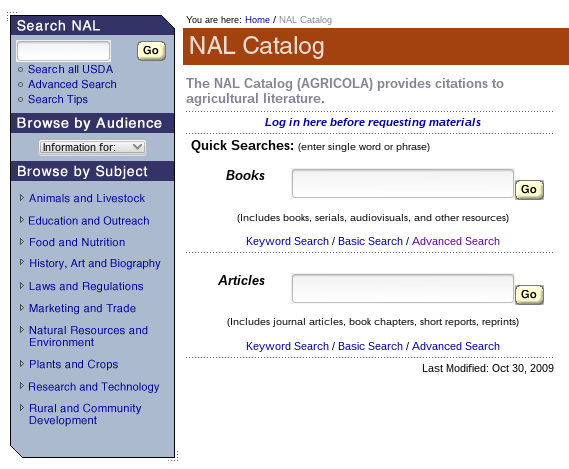
\includegraphics[width=0.5\textwidth]{images/litreview/agricola.png}
\caption{The specific search controls and filters offered by AGRICOLA}
\label{fig:agricola}
\end{figure}

Unfortunately, these domain specific indexing systems usually only contain a
small subset of papers, excluding potentially crucial literature because it
does not quite fit into the subject domain. This problem is often exacerbated
by the decision to leave out some papers and articles because the system
administrators do not have permission from the author or publisher to include
them. The value of these systems to their users is often restricted by the
small proportion of available literature that they index, forcing researchers
to use multiple, domain specific, search engines for their queries.

In contrast, there are also a number of interdisciplinary indexing systems and
online journals such as arXiv( \url{http://arxiv.org/}),
PloSOne(\url{http://plosone.org/}), and JSTOR (\url{http://www.jstor.org/}),
that try to incorporate wide ranges of papers from as many disciplines as
possible. The traits of these systems often complement those of their
domain-specific counterparts; they provide a comprehensive collection of
literature but insufficient filtering and indexing capabilities.

One of the most publicised and well known interdisciplinery scientific
literature search systems is Google Scholar (\url{http://scholar.google.com}).
As can be seen in Figure \ref{fig:scholar_basic}, This is an adaptation of
Google's general search engine to specifically index and search scientific
papers.  Google offers advanced query options specific to Scholar that allow
searching by author, year and for words that occur only in the document title
as shown in figure \ref{fig:scholar_advanced}. Whilst this does deal with the
problem of `information overload' by providing fine control over the
information returned from searches,  the user is still required to have a very
good idea of what they are looking for in terms of keywords and/or specific
authors. It is possible that a user would not know what they are looking for
until they've seen it. Even if the user has a set of keywords to search for,
they can only search the title of the paper or the content as a whole. This
means that users who want to find a particular phrase within a specific
subsection of the paper (e.g.  only look for this phrase in the `Result'
section of the paper) are unable to get results at their desired level of
detail.

\begin{figure}[!hbt]
        \centering
        \begin{subfigure}[b]{0.50\textwidth}
                \centering
                
\includegraphics[width=\textwidth]{images/googlescholar_front.png}
                \caption{Google Scholar's General front page}
                \label{fig:scholar_basic}
        \end{subfigure}%
        \begin{subfigure}[b]{0.50\textwidth}
                \centering
                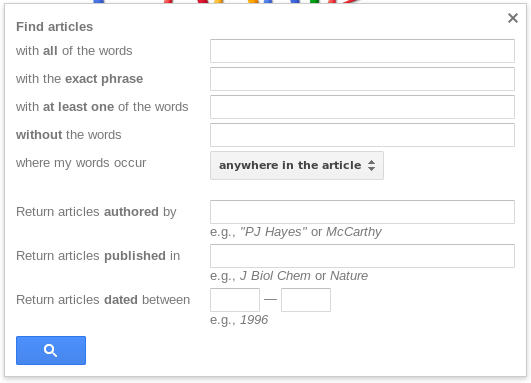
\includegraphics[width=\textwidth]{images/googlescholar_advanced.png}
                \caption{Advanced search features}
                \label{fig:scholar_advanced}
        \end{subfigure}

        \caption{Google Scholar's user interface}
        \label{fig:scholar_interface}
\end{figure}

Search engines such as those discussed above are fairly useful for helping
people to find relevant literature and information when they have some idea of
what they are looking for. However, they demand precision in the use of
keywords and phrases, often leaving researchers looking for literature on highly
specific topics frustrated. Moreover, users can get completely different result
sets by entering synonyms. In comparison, Recommender Systems may perform with
more accuracy and better inclusion when a search term cannot be clearly
defined.

\subsection{Recommender Systems}

Adomavicius and Tuzhilin(2005) define three main types of recommender systems:
Collaborative systems that rely upon \emph{user} data to make recommendations,
Content-based systems that use \emph{content} indexing and feature-extraction
to make recommendations and Hybrid systems that exploit both of these
techniques\cite{adomavicius2005toward}. 

\subsubsection{Collaborative Recommender Systems}

Collaborative Recommender Services like Mendeley
(\url{http://www.mendeley.com/}), ResearchGate
(\url{http://www.researchgate.net/})  and CiteUlike
(\url{http://www.citeulike.org/}) allow users to register their interest in
specific authors and subjects. This allows the sites to build up a profile of
the sorts of materials that its users might be interested in and provide lists
of recommendations.

These systems have the ability to make recommendations to the user without
requiring specific keywords or search terms. They do this by learning the
user's profile and taking into account the preferences of their `friends' and
their browsing history. However, the above-named systems do not take into
account the content of the paper or book. They only deal with the relationships
between users and their reading history. This means that important
discriminatory information that could be contained within the actual document
content is overlooked completely. 

\subsubsection{ Content-based Recommender Systems}

Unlike Collaborative Recommender Systems, which have become commonplace on
today's World Wide Web, there are very few examples of Content-based
Recommender Systems in common use and most of them use metadata. 

More generally, metadata can be said to be extra data that is used to describe
a record but is not contained within it. In the case of literature, metadata is
used to describe attributes of a document such as its title, author and topic.
Although commonly used in content-based recommender systems, metadata does not
contain enough information about its associated document to be used to draw any
meaningful conclusions about whether the paper should recommended. There are
also many discrepancies in the quality of metadata provided by different
scientific journals, thus reducing the reliability of any analysis carried out
on sets of documents from different sources\cite{palepumeta}. A better system
should take into account the content of the whole document.

One example of this comes from Mooney and Loriene(2000) who describe a
content-based book recommender system that use Natural Language Processing
techniques to process full text passages in order to determine similarity
between books\cite{Mooney:2000:CBR:336597.336662}. With a sample of 20,000
books of various genres, this system was found to give accurate
reccomendations. Their work provides an excellent foundation for further
research in this area.

\subsubsection{ Hybrid Recommender Systems }

Hybrid Recommender Systems are designed to combine the Content-based and
Collaboration-based models, employing aspects of both techniques. Huang
\emph{et al.}(2002) describe a graph-based approach to combine content and
collaborative data from books, customers and transactions taken from an online
bookseller\cite{Huang:2002:GRS:544220.544231}. Combining both sources of
information boosted the effectiveness of the recommendation engine and
the system gained improvement with respect to both precision and
recall \emph{(Ibid.).} A scientific literature recommender system could make use
of a similar hybrid technique in order to provide effective recommendations to
researchers.


\subsection{Why Does Partridge Need Natural Language Processing?}

Human literature is generally written in human languages for the consumption of
other humans. Chomsky (1956) defines a hierarchy for the classification of
formal grammars that describe languages \cite{chomsky1956three}. Although it
can be debated where exactly on the hierarchy human language fits (
Reich(1969)\cite{reich1969finiteness} argues that Natural Languages can be
considered finite state and Matthews(1979)\cite{matthews1979grammatical} argues
that Natural Languages cannot even be considered recursively enumerable, cited
in Kornai(1985)\cite{kornai1985natural}) it is clear that they are not in the same
category as most forms of machine language. Literature written for humans must
be interpretted for machines and this is where Natural Language Parsing is
useful.

Natural Language Processing (NLP)  is a branch of Artificial
Intelligence that enables the automated extraction of meaningful information
from texts written in human languages such as French or English. Liddy (2001)
defines Natural Language Processing as:

\begin{quotation} 
A theoretically motivated range of computational techniques for analyzing and
representing naturally occurring texts at one or more levels of linguistic
analysis for the purpose of achieving human-like language processing for a
range of tasks or applications \cite{liddy2001natural}.  
\end{quotation}

Over the last 60 years, NLP has been used in a wide variety of applications
such as automated translation between languages\cite{hutchins2004first}, the
engineering of systems for querying databases using natural languages
\cite{rao2010natural} and for building `chatterbot' systems designed to
communicate with their users in a human-like way\cite{Alfonsi2006}.
More recently, NLP has been used for text classification purposes such as
classifying emotions within phrases and sentences \cite{Wilson05Polarity} and
even within suicide notes \cite{citeulike:11077287}. Laterly, NLP has been
used to detect core scientific concepts within scientific literature.

\subsection{Natural Language Processing in Scientific Papers}
\label{sec:nlpsapienta}

Liakata \emph{et al.} (2012) describe a system for automatically processing and
classifying sentences in a research paper according to the scientific concept
they describe (e.g. a sentence can be categorised as a hypothesis, background
information, a method or similar)\cite{citeulike:10444769}. SAPIENTA
(\url{http://www.sapientaproject.com}) is a machine learning application,
trained using a corpus of physical chemistry and biochemistry research papers
that were manually annotated using the Core Scientific Concepts
(CoreSC)\cite{LIAKATA10.644} scheme. 

CoreSC Liakata \emph{et al.} (2010), derived from earlier work in which Core
Information about Scientific Papers (CISP) is formalised as a way of improving
better metadata for papers\cite{soldatova2007ontology}, is a way to formally
represent core scientific concepts (CoreSC), e.g. background, hypothesis,
method etc., that should be present in scientific articles in a logical
ontology\cite{LIAKATA10.644}. It is implemented as a three layered sentence
based annotation scheme  where annotations are encoded in Extended Markup
Language (XML). CoreSC labels can be allocated to all sentences in a
scientific paper in order to identify which scientific concept each sentence
encapsulates. For example, a sentence with the CoreSC label ``Hypothesis"
conveys some expectation of an experiment or action. An example ``Hypothesis"
identified in a Bioinformatics paper used for testing is:

\begin{quotation}
We assume that, as in the HACA process, condensation is initiated by radical
formation, and then consider reactions of phenyl, naphthyl and anthracenyl with
another PAH to yield for example fluoranthene or
perylene\cite{unterreiner2004reaction}.
\end{quotation}

Alternatively, a ``Background'' CoreSC sentence may refer to prior work or
merely declare a point of interest to the reader. An example from the same
paper is:

\begin{quotation}
The central issue is here the formation of polycyclic aromatic hydrocarbons
(PAHs), which are the main constituents of soot; the PAHs are also health
hazards since they are carcinogenic\cite{unterreiner2004reaction}.
\end{quotation}

An intelligent academic information retrieval system could utilise this
information in order to provide better filtering and search capabilities for
researchers. The ability to search for phrases and keywords by CoreSC would
facilitate context-aware keyword search, that allows researchers to only accept
papers where a term appears in sentences with a specific CoreSC label. This
could be used to greatly improve both the precision with which researchers are
able to perform searches for scientific literature and the accuracy of those
searches in terms of relevance to the reader.

\section{Summary}

After establishing the context and objectives of the Partridge Project, a
number of existing information retrieval and recommendation tools for
scientific literature were examined. A set of academic and general purpose
search engines were critically evaluated; academic search engines found to be
better for precision and general search engines for having a wider variety of
indexed materials. The three core types of recommendation engines,
Content-based, Collaboration-based and Hybrid, were discussed and it was
concluded that much much could be gained through the use of a Hybrid
recommendation system in Partridge. With a clear image of Partridge's
objectives, the next section deals with choosing an effective design
methodology.
